% 経路生成ネットワークの構成（入力画像→畳み込み→行アンカー出力）
% 寸法は vision_planner (version n, 入力 384x640, ROW_START 25) に基づく
\colorlet{netin}{orange!45}
\colorlet{netfm}{black!6}
\newcommand{\slab}[7]{%
  % #1 name, #2 x(left), #3 w, #4 h, #5 depth(projected), #6 fill, #7 label
  \pgfmathsetmacro{\xa}{#2}\pgfmathsetmacro{\xb}{#2+#3}
  \pgfmathsetmacro{\ya}{-0.5*#4}\pgfmathsetmacro{\yb}{0.5*#4}
  \pgfmathsetmacro{\dd}{#5}
  \draw[slab, fill=#6!80!black] (\xa,\yb) -- (\xa+\dd,\yb+\dd) -- (\xb+\dd,\yb+\dd) -- (\xb,\yb) -- cycle;
  \draw[slab, fill=#6!62!black] (\xb,\ya) -- (\xb+\dd,\ya+\dd) -- (\xb+\dd,\yb+\dd) -- (\xb,\yb) -- cycle;
  \draw[slab, fill=#6] (\xa,\ya) rectangle (\xb,\yb);
  \coordinate (#1-w) at (\xa,0);
  \coordinate (#1-e) at (\xb+\dd,0);
  \coordinate (#1-s) at (0.5*\xa+0.5*\xb,\ya);
  \node[dim, below=2pt of #1-s] {#7};
}
\begin{tikzpicture}[
  font=\fontspec{TeX Gyre Heros Cn}\fontsize{8}{8.8}\selectfont,
  >={Stealth[length=1.6mm,width=1.2mm]},
  slab/.style={draw=black!70, line width=0.4pt},
  dim/.style={font=\fontspec{TeX Gyre Heros Cn}\fontsize{7}{7.6}\selectfont, align=center, inner sep=1pt},
  grp/.style={font=\fontspec{TeX Gyre Heros Cn}\fontsize{7.5}{8.4}\selectfont, align=center, inner sep=1pt},
  arr/.style={->, line width=0.5pt},
  brace/.style={draw=black!70, line width=0.4pt}
]
  % ---------- 入力（前面はカメラ画像） ----------
  \slab{in}{0}{1.5}{0.9}{0.08}{netin}{$640\times384$\\3 ch}
  \node[anchor=center, inner sep=0pt] at (0.75,0) {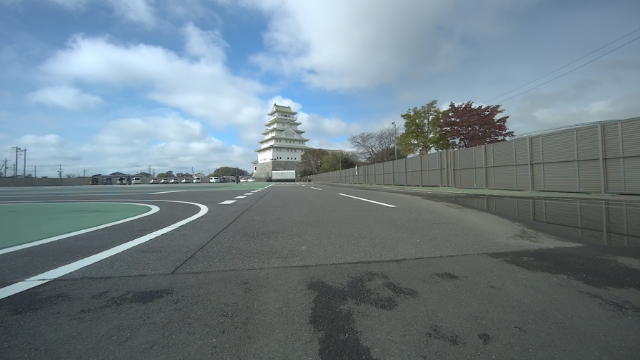
\includegraphics[width=1.5cm,height=0.9cm]{images/example_curve_cam.png}};
  % ---------- バックボーン ----------
  \slab{p1}{1.95}{1.10}{0.66}{0.18}{netfm}{$320\times192$\\16 ch}
  \slab{p2}{3.55}{0.80}{0.48}{0.34}{netfm}{$160\times96$\\64 ch}
  \slab{p3}{4.95}{0.60}{0.36}{0.48}{netfm}{$80\times48$\\128 ch}
  \slab{p4}{6.30}{0.45}{0.27}{0.48}{netfm}{$40\times24$\\128 ch}
  \slab{p5}{7.50}{0.36}{0.20}{0.55}{netfm}{$20\times12$\\256 ch}
  % ---------- ネック ----------
  \slab{n3}{8.80}{0.60}{0.36}{0.34}{netfm}{$80\times48$\\64 ch}
  % ---------- ヘッド ----------
  \slab{h1}{10.10}{0.80}{0.30}{0.34}{netfm}{$160\times23$\\64 ch}
  \slab{h2}{11.55}{0.80}{0.30}{0.08}{netfm}{$160\times23$\\3 ch}
  % ---------- 出力（行ごとの横位置と有無） ----------
  \slab{o1}{12.80}{0.12}{0.60}{0.08}{white}{position\\$23\times3$}
  \slab{o2}{13.75}{0.12}{0.60}{0.08}{white}{existence\\$23\times3$}

  % ---------- 矢印 ----------
  \draw[arr] (in-e) -- (p1-w);
  \draw[arr] (p1-e) -- (p2-w);
  \draw[arr] (p2-e) -- (p3-w);
  \draw[arr] (p3-e) -- (p4-w);
  \draw[arr] (p4-e) -- (p5-w);
  \draw[arr] (p5-e) -- (n3-w);
  \draw[arr] (n3-e) -- (h1-w);
  \draw[arr] (h1-e) -- (h2-w);
  \draw[arr] (h2-e) -- (o1-w);
  \draw[arr] (o1-e) -- (o2-w);

  % ---------- グループ名（下段） ----------
  \draw[brace] (0,-1.25) -- (1.58,-1.25);
  \node[grp, below=1pt] at (0.79,-1.25) {Input image\\(letterboxed)};
  \draw[brace] (1.95,-1.25) -- (8.41,-1.25);
  \node[grp, below=1pt] at (5.18,-1.25) {Backbone\\(convolution, stride 2 at each stage)};
  \draw[brace] (8.80,-1.25) -- (9.74,-1.25);
  \node[grp, below=1pt] at (9.27,-1.25) {Neck\\(upsampling\\and fusion)};
  \draw[brace] (10.10,-1.25) -- (12.43,-1.25);
  \node[grp, below=1pt] at (11.27,-1.25) {Head\\(row anchors; softmax over\\160 columns in each row)};
  \draw[brace] (12.80,-1.25) -- (13.95,-1.25);
  \node[grp, below=1pt] at (13.37,-1.25) {Output\\(3 paths $\times$\\23 rows)};

  % ---------- 出力のイメージ（画像上の行アンカーと 3 本の経路） ----------
  \begin{scope}[shift={(14.6,-0.8)}]
    \draw[slab, fill=white] (0,0) rectangle (2.3,1.6);
    % 地平線より下に行アンカー
    \foreach \k in {0,...,7} {
      \draw[black!35, line width=0.3pt, dash pattern=on 1pt off 1pt] (0,{0.12+0.15*\k}) -- (2.3,{0.12+0.15*\k});
    }
    \draw[black!60, line width=0.3pt] (0,1.35) -- (2.3,1.35);
    \node[dim, anchor=south west, inner sep=0.5pt] at (0.02,1.36) {horizon};
    % straight: 下中央から消失点へ
    \draw[blue!70!black, line width=0.7pt] (1.15,0.12) -- (1.15,1.2);
    \foreach \k in {0,...,7} { \fill[blue!70!black] (1.15,{0.12+0.15*\k}) circle (0.5pt); }
    % left
    \draw[green!55!black, line width=0.7pt] (1.15,0.12) .. controls (1.1,0.55) and (0.75,0.8) .. (0.15,0.95);
    \foreach \k in {0,...,5} { \fill[green!55!black] ({1.15-0.2*\k*\k/5},{0.12+0.15*\k}) circle (0.5pt); }
    % right
    \draw[orange!85!black, line width=0.7pt] (1.15,0.12) .. controls (1.2,0.55) and (1.55,0.8) .. (2.15,0.95);
    \foreach \k in {0,...,5} { \fill[orange!85!black] ({1.15+0.2*\k*\k/5},{0.12+0.15*\k}) circle (0.5pt); }
    \node[dim, text=green!55!black, anchor=south west, inner sep=0.5pt] at (0.02,0.98) {left};
    \node[dim, text=blue!70!black, anchor=south west, inner sep=0.5pt] at (1.2,1.17) {straight};
    \node[dim, text=orange!85!black, anchor=south east, inner sep=0.5pt] at (2.28,0.98) {right};
    \node[grp, below=1pt] at (1.15,-0.45) {Row anchors and the\\horizontal position\\of each path};
  \end{scope}
  \draw[arr] (o2-e) -- (14.6,0);
\end{tikzpicture}
